
%(BEGIN_QUESTION)
% Copyright 2011, Tony R. Kuphaldt, released under the Creative Commons Attribution License (v 1.0)
% This means you may do almost anything with this work of mine, so long as you give me proper credit

Sketch the necessary tube and wire connections to calibrate this DP transmitter, using a deadweight tester as the standard pressure source.  The transmitter requires at least 14 volts in order to properly function:

\vskip 10pt

$$\includegraphics[width=15.5cm]{i03564x01.eps}$$

Be sure to note the following details as well:

\begin{itemize}
\item{} Proper mode of loop calibrator ({\it Read}, {\it Simulate} (``2-Wire''), or {\it Source})
\item{} Proper manifold valve positions ({\it open} versus {\it closed})
\end{itemize}

\underbar{file i03564}
%(END_QUESTION)





%(BEGIN_ANSWER)

\noindent
2 points for proper tube connections; 2 points for proper wire connections; 1 point for each proper valve position; 2 points for proper caibrator mode (either {\it read} if connected in series with the batteries or {\it source} if connected without the batteries):

$$\includegraphics[width=15.5cm]{i03564x02.eps}$$

%(END_ANSWER)





%(BEGIN_NOTES)

{\bf This question is intended for exams only and not worksheets!}.

%(END_NOTES)


